%2S необходимо литературу проставить, оригинальная статья тут materials/gesdev2017/genesdev2017.pdf
%2S нужно перевести вот эту картинку https://docs.google.com/drawings/d/1Wa7FAkYUa-TmG-6vC0wwXJO0_HeVc04UCN8hmnvNM7I/edit

\subsection{Введение}
Кинетохоры представляют собой большие субклеточные структуры из $\sim$75 полипептидов, которые собираются на центромерах хромосом, чтобы сделать возможным точное разделение реплицированных дочерних хромосом во время деления клеток \cite{fukagawa_centromere_2004,biggins_composition_2013}. Открытие трех центромер-специфичных аутоантигенов человека, обозначенных CENP-A (гистоновый вариант CenH3), CENP-B (специфичный для последовательности фактор связывания ДНК спираль-виток-спираль) и CENP-C (компонент внутреннего кинетохора), проложили путь к пониманию центромерного хроматина на молекулярном уровне и его роли в сборке кинетохор \cite{fukagawa_centromere_2014}. На фундаментальном уровне нуклеосомы замена канонического гистона H3 на CENP-A в специфичных для центромеры нуклеосомах создает платформу для рекрутирования CENP-C \cite{carroll_dual_2010,gascoigne_induced_2011}. CENP-C колокализуется с CENP-A на центромерах многоклеточных животных и служит структурной связи между нуклеосомами CENP-A и белками внешней кинетохоры, тем самым соединяя центромеры с микротрубочками для сегрегации хромосом \cite{moroi_autoantibody_1980,earnshaw_identification_1985,saitoh_cenp-c_1992,sullivan_determining_2001,biggins_composition_2013}. CENP-C является ключевым компонентом мультисубъединичного комплекса CCAN (конститутивной сеть, ассоциированная с центромерой), образующего внутреннюю часть кинетохоры \cite{weir_insights_2016}. Следовательно, молекулярные основы взаимного узнавания между CENP-C и нуклеосомой CENP-A является центральным фактором для понимания того, как внутренняя кинетохора взаимодействует с центромерным хроматином.

Центральная часть полипептида CENP-C содержит три консервативных домена, важных для узнавания центромеры: высококонсервативный ``сигнатурный мотив CENP-C'', который контактирует с гидрофобным C-концом CENP-A \cite{carroll_dual_2010,kato_conserved_2013}, центральная ДНК-связывающая область, которая содержит CENP-C-подобный мотив, и домен гомодимеризации \cite{brown_sequence_1995,yang_identification_1996,sugimoto_characterization_1997,politi_cenp-c_2002,milks_dissection_2009,trazzi_c-terminal_2009}. У почкующихся дрожжей, гомолог CENP-C Mif2 \cite{meeks-wagner_isolation_1986} не обладает специфической для позвоночных ДНК-связывающей областью, но он содержит один мотив CENP-C и один ``AT-крюк'' \cite{brown_sequence_1995,huth_solution_1997,reeves_structure_2000}. Ранние исследования показали, что AT-крюк в Mif2 способствует узанванию центромер и сегрегации хромосом \textit{in vivo} \cite{brown_sequence_1995,lanini_domains_1995,meluh_evidence_1995,cohen_structural_2008}. Более того, N-концевой домен в Mif2 ассоциируется с двумя кинетохорными белками (Ame1-Okp1), чтобы облегчить сборку внешних кинетохор \cite{hornung_cooperative_2014}.

\subsection{Построение модель взаимодействия на основе данных футпринтинга ДНК}
Для понимания взаимодействия Mif2 с центромерными нуклеосомами \textit{in vitro} была проведена серия экспериментов по футпринтингу комплексов гидроксильными радикалами. Для обработки и интерпретации данных была применена программа HYDROID описанная в главе \ref{part5_hrf}, а также построенная нами и описанная в той же главе модель центромерной нуклеосомы.

ДНК центромеры дрожжей длиной 125 п.н. состоит из трех смежных генетических элементов: CDEI, CDEII и CDEIII \cite{hegemann_centromere_1993}. Мы использовали метод футпринтинга ДНКазой I для определения сайта связывания димера Mif2c на нуклеосоме Cse4/CEN3 -- участка длиной  $\sim$30 п.н. в пределах AT-богатого элемента CDEII ($\sim$85 п.н.) на одной стороне от диады нуклеосомы в направлении CDEIII. Для дальнейшего картирования точных контактов Mif2-ДНК мы выполнили футпринтинг димера Mif2c на нуклеосоме Cse4/CEN3 методом гидроксильного футпринтинга. Поскольку гидроксильный радикал представляет собой небольшую молекулу, от его атаки защищены только места тесных контактов. Как показано на рисунке  \ref{fig:p6_5_f5}, димер Mif2c защищает $\sim$30 п.н. ДНК от расщепления гидроксильным радикалом, что в высокой степени согласуется с защитой от ДНКазы I. Учитывая, что минимальный сайт для связывания  Mif2 лишенного димеризационного домена составляет 16-18 п.н., защита в 30 п.н. при связывании димера Mif2c предполагает, что оба ДНК-связывающих домена из димерного Mif2 взаимодействует с одной стороной нуклеосомы.

Это поднимает вопрос, почему димер Mif2 должен связываться только с одной стороной нуклеосомы, когда обе стороны состоят примерно из эквивалентного процента AT. Мы исследовали эту проблему и обнаружили второй, более медленный по подвижности в геле комплекс при двукратном или трехкратном увеличении концентрации димера Mif2c в реакции связывания. Анализ гидроксильным футпринтингом показывает, что обе стороны нуклеосомной диады этого комплекса теперь защищены от расщепления гидроксильными радикалами (данные не показаны). Таким образом, одна нуклеосома Cse4 / CEN3 способна связываться с двумя димерами Mif2, занимающими каждую сторону нуклеосомы. Связывание с AT-богатой ДНК является доминирующим фактором, но правила предпочтительного связывания со специфической AT-богатой последовательностью остаются неясными. Мы предполагаем, что точное расположение пары оснований AT может придавать тонкие различия в гибкости и / или конформации ДНК, делая одну AT-богатую сторону от диады более привлекательной, чем другую.

Чтобы определить, является ли сайт между диадой нуклеосомы и CDEIII  предпочтительным для взаимодействий Mif2 на других центромерных нуклеосомах, мы выполнили эксперименты по футпринтингу нуклеосом, реконструированных на CEN10. Интересно, что сайт связывания димера Mif2c был картирован в AT-богатых регионах на противоположной стороне от нуклеосомной диады для CEN10, по направлению к CDEI. Таким образом, Mif2 взаимодействует с нуклеосомой Cse4 в соседнем с диадой сайте внутри CDEII, но его ориентация связывания относительно оси диады, по-видимому, специфична для каждой конкретной центромеры. Это означает, что определенные паттерны последовательности лежащей в основе AT-богатой ДНК предпочтительнее для Mif2. Чтобы проверить, отражают ли  области повышенной защиты, наблюдаемые в нуклеосомах при связывание димера Mif2c, какие-либо свойства ДНК самой по себе, мы выполнили реакции футпринтинга ДНКазы I с голой ДНК CEN3. Мы не наблюдали никаких специфических следов связывания для димера Mif2c на голой ДНК CEN3. Это указывает на то, что сайт-специфическая локализация Mif2 на нуклеосоме требует вовлечения как ДНК, так и гистоновых сигналов Cse4.

\begin{figure}[H]
    \centering
    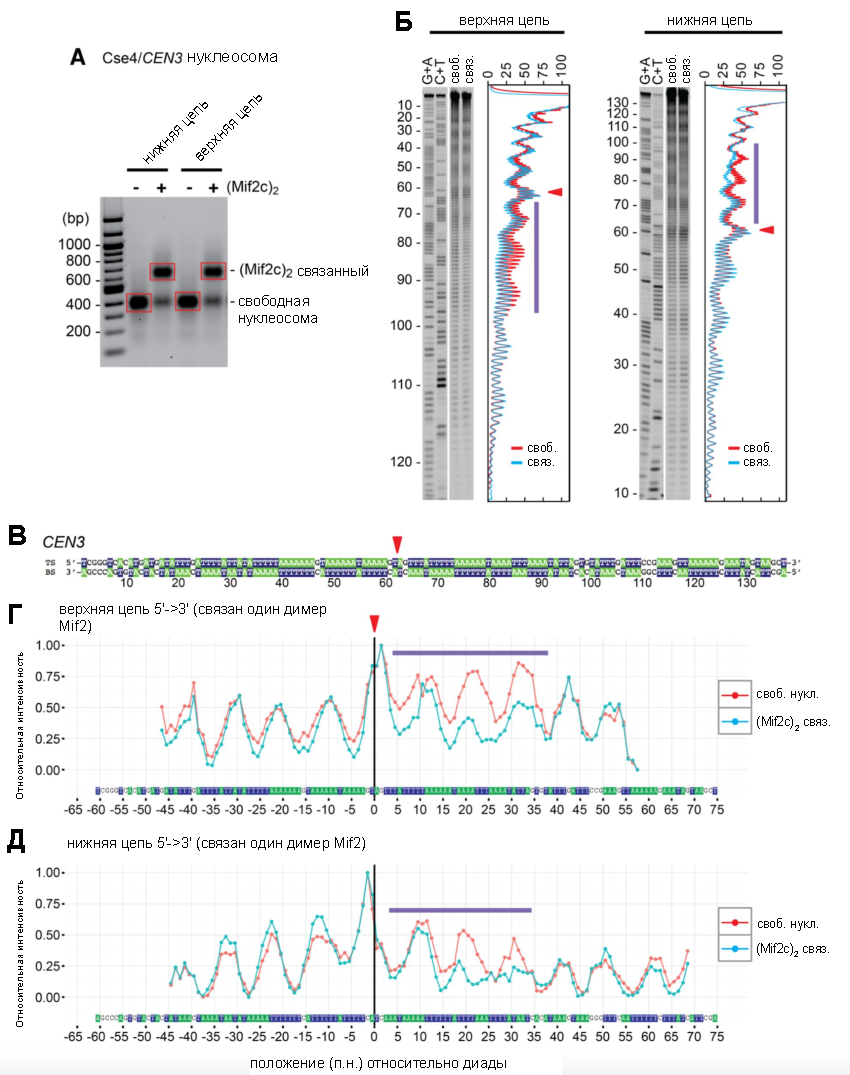
\includegraphics[width=0.9\textwidth]{images/p6/p6_4/p6_5_f5.pdf}
    \caption[Анализ комплексов димеров Mif2 с центромерными нуклеосомами Cse4/CEN3 методами гидроксильного футпринтинга]{Анализ комплексов димеров Mif2 с центромерными нуклеосомами Cse4/CEN3 методами гидроксильного футпринтинга. (A) Анализ комплексов с помощью агарозного гель электрофореза после расщепления ДНК гидроксильными радикалами. (Б) Изображения продуктов реакции после ПААГЭ. Красные линии  - нуклеосомы, голубые - нуклеосомы с димером Mif2c. (В) Положение  диады на ДНК для Cse4/CEN3 нуклеосомы (см. главу \ref{part5_hrf}). (Г, Д) Профили интенсивности расщепления гидроксильными радикалами цепей ДНК в нуклосомах с и без Mif2. Фиолетовые линии - дополнительная защита от расщепления.}
    \label{fig:p6_5_f5}
\end{figure}

\subsection{Обсуждение}
Понимание работы центромер многоклеточных животных представляют собой некоторый парадокс, потому что их последовательности сильно расходятся даже между родственными видами, несмотря на функциональную законсервированность \cite{henikoff_centromere_2001}. Неуловимая природа универсального паттерна последовательности повторяющихся ДНК активных центромер многоклеточных животных привела к широкому признанию того, что идентичность центромер управляется эпигенетическими механизмами; т.е. за счет сборки и свойств унаследованного гистона CENP-A, а не лежащей в основе последовательности ДНК центромеры \cite{sullivan_determining_2001,allshire_epigenetic_2008,black_epigenetic_2011}. Заметным исключением является строго генетически определенная позиция центромер почкующихся дрожжей, где нуклеосомный гистон Cse4/CENP-A деградирует при переходе G1 – S каждого клеточного цикла, что исключает эпигенетическую передачу \cite{biggins_composition_2013,wisniewski_imaging_2014}. Вместо этого центромерный хроматин восстанавливается \textit{de novo} с помощью инструкций от трех специфических элементов последовательности (120 п.н.) центромеры дрожжей и их множественных родственных факторов \cite{westermann_structures_2007}. Интересно, что ранее существовавший Mif2 на центромере почкующихся дрожжей передается дочерним клеткам; значение этой передачи еще предстоит изучить.

В этой работе мы выделили отличительные особенности AT-богатой центромеры дрожжей ДНК. Варианты как ДНК, так и гистонов вносят вклад в тысячукратное усиление связыания Mif2 с центромерными нуклеосомами по сравнению с перицентромерным. Это огромное предпочтение, вероятно, лежит в основе сайт-специфичности нуклеации кинетохор, хотя другие механизмы могут вносить свой вклад; напр. взаимодействия с участием N-концевого хвоста Cse4 \cite{chen_n_2000,samel_methylation_2012} и взаимодействия между N концом Mif2 и кинетохорными компонентами CENP-UAme1-CENP-QOkp1 \cite{hornung_cooperative_2014}. Дальнейший вклад в селективность нуклеосом CENP-A по сравнению с нуклеосомами H3 может также происходить от компонентов CCAN \cite{weir_insights_2016}.

Мы подтвердили важность Cse4-гидрофобного С-конца для взаимодействий Mif2, что согласуется с предыдущими исследованиями \cite{carroll_dual_2010,guse_vitro_2011,kato_conserved_2013}. Однако, хотя вклад гистоновых фолдов CENP-A ранее был исключен \cite{guse_vitro_2011}, мы обнаружили явную важность петли L1, несущей три дополнительных заряженных и полярных остатка (KDQ), и спирали $\alpha$-2 Cse4. Однако, как мы показали весьма важной является и вклад последовательности ДНК в связывание Mif2. Какие особенности  AT-богатой CDEII последовательности длиной 85-п.н. способствуют связыванию Mif2? Область защиты ДНК от расщепления гидроксильными радикалами длиной $\sim$30 п.н., возникающая в результате связывания димера Mif2, покрывает большую часть одной AT-богатой стороны нуклеосомы. CDEII для всех 16 центромер дрожжей содержат несколько коротких участков An$\cdot$Tn или Tn$\cdot$An трактов плюс динуклеотидные шаги ApT или TpA между участками. Длина и расположение трактов различаются между центромерами \cite{baker_genetic_2005}. Тракты An$\cdot$Tn и Tn$\cdot$An обладают узкой малой бороздкой, большим пропеллерным разворот оснований (propeller twist), а также бифуркационными водородными связями, которые улучшают стэкинг оснований и жесткость спирали \cite{coll_bifurcated_1987,nelson_structure_1987}. С другой стороны, шаги динуклеотидов TpA (но не шаги ApT) обнаруживают расширенные малые бороздки на стыках трактов \cite{stefl_dna_2004}. Одна из этих или обе геометрические особенности AT-богатой ДНК могут изменять обычные спиральные параметры нуклеосомной ДНК, намотанной на гистоновое ядро (Bishop et al. 2011). Например, кристаллическая структура одного длинного тракта A16$\cdot$ T16 на канонической нуклеосоме выявила локальное искажение спирали нуклеосомной ДНК \cite{bao_nucleosome_2006}.

Учитывая корреляцию между предпочтением связывания Mif2 и AT-богатым составом ДНК, мы предполагаем, что конформации AT-богатого CDEII распознаются AT-крюк и кластерами аминокилот аргинина и лизина (RK) Mif2. Mif2 имеет один классический AT-крюк (GRPRGRPK) на С-конце своего ДНК/гистон связывающего домена. Структурные исследования показали, как отдельные остатки AT-крюков взаимодействуют с узкими малыми бороздками родственных AAAT и AATT элементов \cite{reeves_t-dna-binding_1990,huth_solution_1997,reeves_structure_2000}. Аргинины и, в меньшей степени, лизины кластеров RK широко используются для во взаимодействии белок-ДНК не только гистонового ядра нуклеосомы \cite{luger_crystal_1997}, но также и факторов транскрипции, специфичных для последовательности животных, таких как как UBX, OCT1, бактериальный репрессор MogR \cite{rohs_role_2009,rohs_origins_2010,shen_recognition_2009,kong_functional_2015}. Мы предполагаем, что кластеры RK, используют этот способ взаимодействия с ДНК как часть своей стратегии по специфическому связыванию. Мы предполагаем, что наши результаты закладывают важные основы для дальнейших исследований и уточнению структурно-динамической модели взаимодействия Mif2 с центромерными нуклеосомами.